\chapter{Problems with Virtual Container Networks}
\label{chap:research}
%\emph{This chapter reports on the execution of the research method as described in an earlier chapter. If the research has been divided into phases, they are introduced, reported on and concluded individually. If needed, this chapter could be split up to balance out the sizes of all chapters.}
 First we list the features are required by operators to manage virtual networks in Section~\ref{sec:required-features}, secondly we explain the current difficulties with managing virtual networks on \gls{dcos} in Section~\ref{sec:current-state}. Next we present the approach taken by another popular container orchestration platform, Kubernetes, to handle virtual networks in Section~\ref{sec:k8s-virtual-networks}. To finish we provide an overview of the problems at the end of this chapter in Section~\ref{sec:problems}.

\section{Required features}
\label{sec:required-features}
We came up with a list of required features that an operator should be able to execute to manage virtual networks and policies on a container orchestration platform. Below is the list of the features with an accompanying explanation from the viewpoint of an operator of the cluster. As an operator I want to:
\begin{itemize}
    \item[\textit{list virtual networks:}] to see which networks are available in my cluster and see properties such as the name, tags, subnets and available IP addresses.
    \item[\textit{select virtual network:}] to select a virtual network to launch my workload on.
    \item[\textit{create virtual network:}] to provision and create new virtual networks in my cluster without manually configuring every agent in the cluster.
    \item[\textit{list network policies:}] to get an overview of all the configured network policies in the cluster, which can be filtered based on service, tenant or label to search for specific rules that are blocking traffic.
    \item[\textit{create network policy:}] to apply new firewall policies in the cluster without worrying about the different implementations of different plugin vendors.
    \item[\textit{know the available IPv4 addresses:}] to determine if the solution is usable for the number of services in the cluster.
    \item[\textit{have IPv6 support:}] to allow for native IPV6 support for my services and a bigger pool of available IP address for the growing number of applications with their own IP address.
\end{itemize}

\section{Current state of virtual networks in DC/OS}
\label{sec:current-state}
\Gls{dcos} provides virtual networks by itself as overlay networks which can be used by the Docker and Mesos containerizer. This overlay is prepacked and enabled by default on the cluster. \Gls{cni} plugins are also supported on \gls{dcos} and can be used by both containerizers. There are three different networking modes available for containers on \gls{dcos}:
\begin{itemize}
    \item[\textbf{Host networking}] The container shares the same network namespace as the host, this restricts the ports an application can use as the TCP/UDP port range is shared with the host.
    \item[\textbf{Bridge networking}] The container is launched on a bridge interface, has its own network namespace and applications are only reachable over port mappings to the host.
    \item[\textbf{Container networking}]  The container has its own network namespace and the underlying network is provided by \gls{cni} plugins. This networking mode is the most flexible as it allows operators to run applications on any port without dealing with port conflicts or port mappings.
\end{itemize}

\subsection{DC/OS virtual networks}
\label{subsec:dcos-virtual-networks}
The overlay network was introduced to enable an IP-per-container model in \gls{dcos}. This allows operators to run applications on the default ports without worrying about port conflicts. This is done by creating an overlay network using \gls{vxlan}\cite{mahalingam2014virtual} which is supported by the Linux kernel. It works by creating two network bridges on each host, one for each containerizer. Containers on the same host and bridge can communicate directly with each other over the network bridge. A packet from a Mesos container to a Docker container on the same host will be routed through both bridges. A packet from a Mesos container on Agent~1 to a Docker container on Agent~2 follows a different path. First the packet will be routed to the Mesos bridge, the host's network stack consumes the package and encapsulates using \gls{vxlan} on Agent~1. Next Agent~2 decapsulates this packet and sends it up to the Docker bridge to be sent to the Docker container as can be seen in Figure~\ref{fig:dcos-overlay-arch}. A container gets assigned a virtual network interface with the help of the \gls{dcos} overlay \gls{cni} plugin.

\begin{figure}
    \centering
    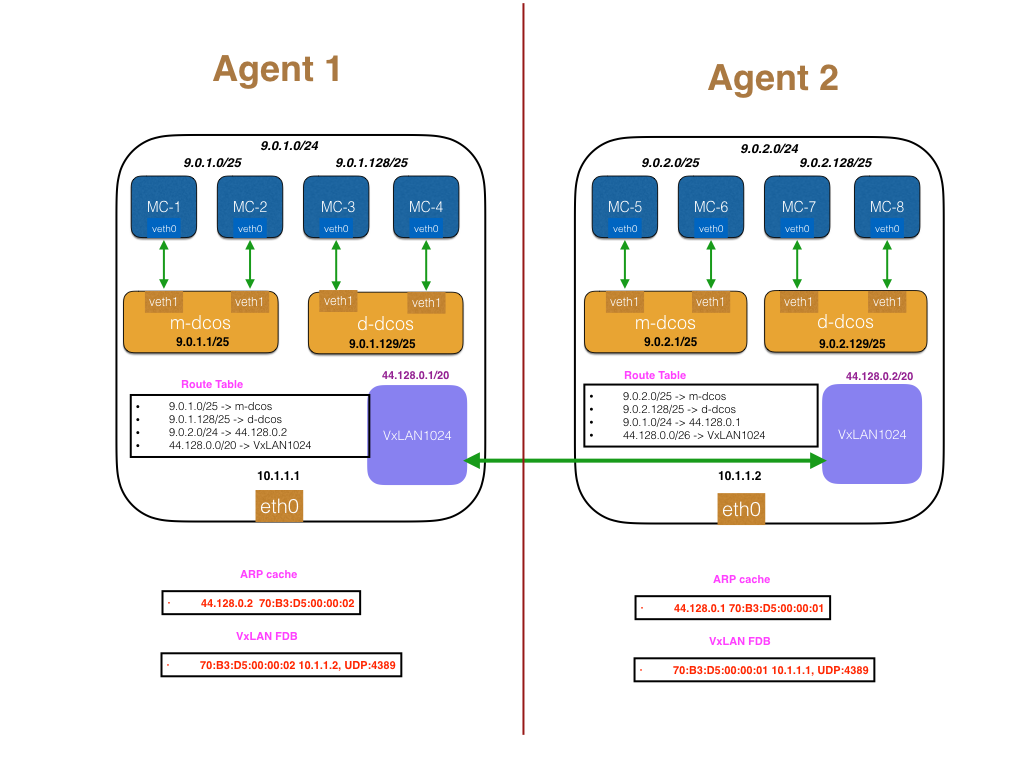
\includegraphics[width=1\columnwidth]{images/dcos-overlay-arch}
    \caption{DC/OS overlay in action\cite{dcos_overlay_arch}}
    \label{fig:dcos-overlay-arch}
\end{figure}

IP addresses are managed by the agent itself instead of a central location. A central location would require a reliably and consistent way of IP address assignment to containers in the cluster. The default configuration uses a \texttt{9.0.0.0/8} subnet, this subnet is divided in smaller chunks: a \texttt{/24} to be managed by every agent itself. On the agent this subnet is divided into two equal subnets for each containerizer, resulting in 32 usable IP addresses for each container type on every agent. The agent's overlay module can request its allocated subnet from the overlay module running on the masters based on its identifier. To launch a container on a virtual network an operator can select the required virtual network from the \gls{dcos} web interface when configuring a task as \gls{dcos} is aware of the default overlay networks.

The default overlay network currently has the following limitations:
\begin{itemize}
    \item A limit on the number of usable IP addresses on each host, determined by the network prefix size. The default maximum is 32 Mesos and 32 Docker containers.
    \item Only IPv6 support for Docker containers, Mesos containers will fail to start as the overlay network does not support IPv6 for Mesos containers.
    \item Operators are only able to create and delete virtual networks during the installation of the cluster.
    \item The length of network names is limited to 15 characters by the Linux kernel.
    \item Marathon cannot execute health checks in the default configurations as Marathon itself is not running on the virtual network.
    \item No \gls{api} to create and manage network policies on the virtual networks.
\end{itemize}

\subsection{CNI plugins on DC/OS}
\label{subsec:dcos-cni}
To allow for more flexibility with virtual networks on \gls{dcos}, operators can also chose to create virtual networks with other providers. Plugins following the \gls{cni} specification as discussed in Section~\ref{sec:cni} can be installed on \gls{dcos}. This works by placing the plugin in a dedicated folder on every agent. Networks can be created and configured by placing their relevant configuration files on every agent. Plugin location: \texttt{/opt/mesosphere/active/cni/} and configuration location: \texttt{/opt/mesosphere/etc/dcos/network/cni/}. A restart of the Mesos agent is required to make use of the new plugin or new configuration. The method mentioned above is only possible when using the Mesos containerizer. For Docker we need to create a Docker network on every agents with the \gls{cni} plugin as its driver.

Next any container can be launched on a virtual network by adding the following JSON to the configuration of the application: \texttt{\{"ipAddress": \{"networkName": "<<name>>"\}\}}. This will instruct the Mesos scheduler to request an IP address from that network using the configured \gls{cni} plugin. The plugin will take care of \gls{ipam} and creating and deleting of the network interface on the host machine. Depending on the features of the \gls{cni} plugin, network policies can be applied by using the \gls{api} of the plugin.

The \gls{cni} plugin model for \gls{dcos} makes it flexible for operators to configure different virtual networks. However there is a drawback to this approach, as these networks are not visible to the operators and users of the cluster, as stated on the documentation\cite{dcos_sdn}:
\begin{displayquote}
    ``NOTE: The network tab currently displays information about containers that are associated with virtual networks managed by DC/OS overlay. It does not have information about containers running on virtual networks managed by any other CNI/CNM provider.'' 
\end{displayquote}
This makes it confusing for developers who want to deploy their applications. Colleagues on the client's project are having a hard time to understand how their applications are deployed and how to connect to them. Containers now live on a different network and are not always available on every machine. For example the SSH jumpbox used to connect to the cluster is not setup with Calico and is unaware of the virtual networks. It does not have the routes in its route table to connect to the container workloads on a virtual network. 

There is also a problem with the different types of \gls{dns} providers within \gls{dcos}. The mesos-dns component provides a \gls{fqdn} to every service with the following structure: \texttt{<service-name>.<group-name>.<framework-name>.mesos}. This domain name however returns the IP address of the host of the container. In the case that the container is running on a virtual network it will return the wrong IP address. A connection is not possible because the port is only in use on the container network interface, resulting in a time-out for a user request. It is possible with a non recommended workaround to instruct Mesos to return the container IP address instead of the host IP address\cite{mesos_workaround}. The other and newer \gls{dns} provider is dcos-dns providing different addresses based on the network type of the container, these entries are summarised in Table~\ref{tab:dcos-dns} together with the mesos-dns.

\begin{table}[ht]
\centering
\begin{tabular}{l l l} 
 \textbf{DNS name} & \textbf{Container IP} & \textbf{Host IP} \\
 \hline\hline
 \texttt{*.autoip.dcos.thisdcos.directory} & Container networking & Host or bridge networking \\ 
 \texttt{*.agentip.dcos.thisdcos.directory} & & \checkmark \\
 \texttt{*.containerip.dcos.thisdcos.directory} & \checkmark & \\
 \texttt{*.mesos} & \checkmark & \\
 \hline
\end{tabular}
\caption{Different DNS entries for \gls{dcos} tasks}
\label{tab:dcos-dns}
\end{table}

To summarise we have the following drawbacks of using \gls{cni} plugins on \gls{dcos} to create virtual networks:
\begin{itemize}
    \item No method to retrieve or select the virtual networks created with \gls{cni} in the \gls{dcos} web and command line interface. Operators can specify a virtual network name for a container to attach it to that network, however there is no place to see the available networks created with \gls{cni} plugins.
    \item No generic method of configuring network policies, as each plugin provider has its own dedicated \gls{api}.
    \item An operator manually has to distribute the plugin and configuration files to every slave using a custom build solution.
    \item Different \gls{dns} providers return different IP addresses for container workloads on a virtual network.
\end{itemize}

\section{Virtual networks in Kubernetes}
\label{sec:k8s-virtual-networks}
There are different ways of connecting containers in Kubernetes. The most basic one is in a pod where containers in the same pod can communicate via localhost. Pods get their own unique IP address, called the IP-per-pod model, preventing operators to deal with port mappings and \gls{nat} to connect to pods from another pod or host. This network can be implemented by a \gls{cni} plugin or other available\gls{sdn} solutions\cite{k8s-network} which are available in Kubernetes. Furthermore if a plugin supports network policies an operator can leverage the plugin to configure network policies in the cluster. All the virtual network related options can be configured using the kube-apiserver as discussed in Section~\ref{subsec:kubernetes}, such as configuring the network provider and managing its network policies regardless of the chosen implementation. This makes it easy and transparent to the operators of a Kubernetes cluster.

To connect to a pod, from another pod or externally through a load balancer, we cannot use the pod IP address as this IP can change when pods are being rescheduled by the scheduler or when we have a set of the same pods for high availability. We can define a service which uses the kube-proxy, which is present on every node, to route the requests to the right set of pods. By default traffic from the client is captured by iptables\cite{iptables} on the host and redirected to be forwarded by the kube-proxy.

\section{Problems with virtual networks on DC/OS}
\label{sec:problems}
In the first section of this chapter we showed that operators can choose to launch a container on a virtual network provided by \gls{dcos}. Using the default overlay network, operators can select the network from the web interface as \gls{dcos} is aware of the networks that have been created with the overlay module. However this is not the case with virtual networks provided by \gls{cni} plugins. Table~\ref{tab:problems} gives an overview of the virtual network related features available in \gls{dcos} and Kubernetes. As you can see Kubernetes does provide most of the features already as it stores the network state with the kube-apiserver.

\begin{table}
\centering
\renewcommand*{\arraystretch}{1.4}
\begin{tabular}{|p{4cm}|p{2.5cm}|p{4cm}|p{2.5cm}|}\hline 
 \textbf{Feature} & \textbf{\gls{dcos} overlay networks} & \textbf{\gls{dcos} \gls{cni} plugins} & \textbf{Kubernetes}\\ \hline
 \textit{List virtual networks} & Available & Operator has to manual inspect the \gls{cni} configuration files on every host & Available \\ \hline
 \textit{Select virtual network} & Available & Operator has to manual provide a virtual network name based on the list obtained from above & Available \\ \hline
 \textit{Create virtual network} & Only at installation time & Manual on every host & Available \\ \hline
 \textit{List network policies} & Network policies are not provided & Operator has to use the plugin specific \gls{api}  & Available \\ \hline
 \textit{Create network policy} & Network policies are not provided & Operator has to use the plugin specific \gls{api} & Available \\ \hline
 \textit{Available IPv4 addresses} & 32 per containerizer per host & Plugin specific & Plugin specific \\ \hline
 \textit{IPv6 support} & Only for Docker containers & Plugin specific & Plugin specific \\ \hline
\end{tabular}
\caption{Available features for virtual container networks}
\label{tab:problems}
\end{table}
